\section{Results}
\label{sec:results}

We organize results around the five hypotheses. Across the board, the intervention fails: it is
near the bottom on absolute ratings (\secref{sec:res-absolute}), loses every pairwise comparison
on overall quality (\secref{sec:res-pairwise}), adapts to the reader \emph{least}
(\secref{sec:res-adapt}), and is the most homogenized and most expensive condition
(\secref{sec:res-cost}). The ordering replicates with a second generator
(\secref{sec:res-replication}). Throughout, \simtom---a one-shot audience model---is the best
condition.

\subsection{Absolute audience ratings (H1)}
\label{sec:res-absolute}

\Tabref{tab:absolute} reports the audience model's ratings while role-playing the reader.
\persentence is near the bottom on every dimension, barely above \plain and clearly below both
\cot and \simtom. Paired Wilcoxon tests (intervention vs.\ each baseline), Holm-corrected, show
\persentence is significantly \emph{worse} than \simtom on fit ($p=0.0001$), engagement
($p=0.0002$), and understanding ($p=0.057$), and worse than \cot on fit ($p=0.0007$) and
engagement ($p=0.0025$); it is statistically indistinguishable from \plain. The proposed
intervention thus fails to improve audience fit---\textbf{H1 is refuted}
(\figref{fig:absolute}).

\begin{table}[t]
\centering
\caption{Absolute audience ratings (\gemini role-playing the reader, $1$--$10$; $n=60$; higher is
better). \persentence, the intervention, is near the bottom on every dimension---below both
reasoning baselines and only marginally above \plain. \simtom is best throughout. Best results in
\textbf{bold}.}
\label{tab:absolute}
\begin{tabular}{@{}lcccc@{}}
\toprule
\textbf{Metric} & \plain & \cot & \simtom & \persentence \textit{(ours)} \\
\midrule
Audience-fit   & 6.37 & 7.12 & \textbf{7.28} & 6.52 \\
Engagement     & 5.80 & 6.45 & \textbf{6.62} & 5.93 \\
Understanding  & 9.15 & 9.30 & \textbf{9.32} & 9.08 \\
\bottomrule
\end{tabular}
\end{table}

\begin{figure}[t]
\centering
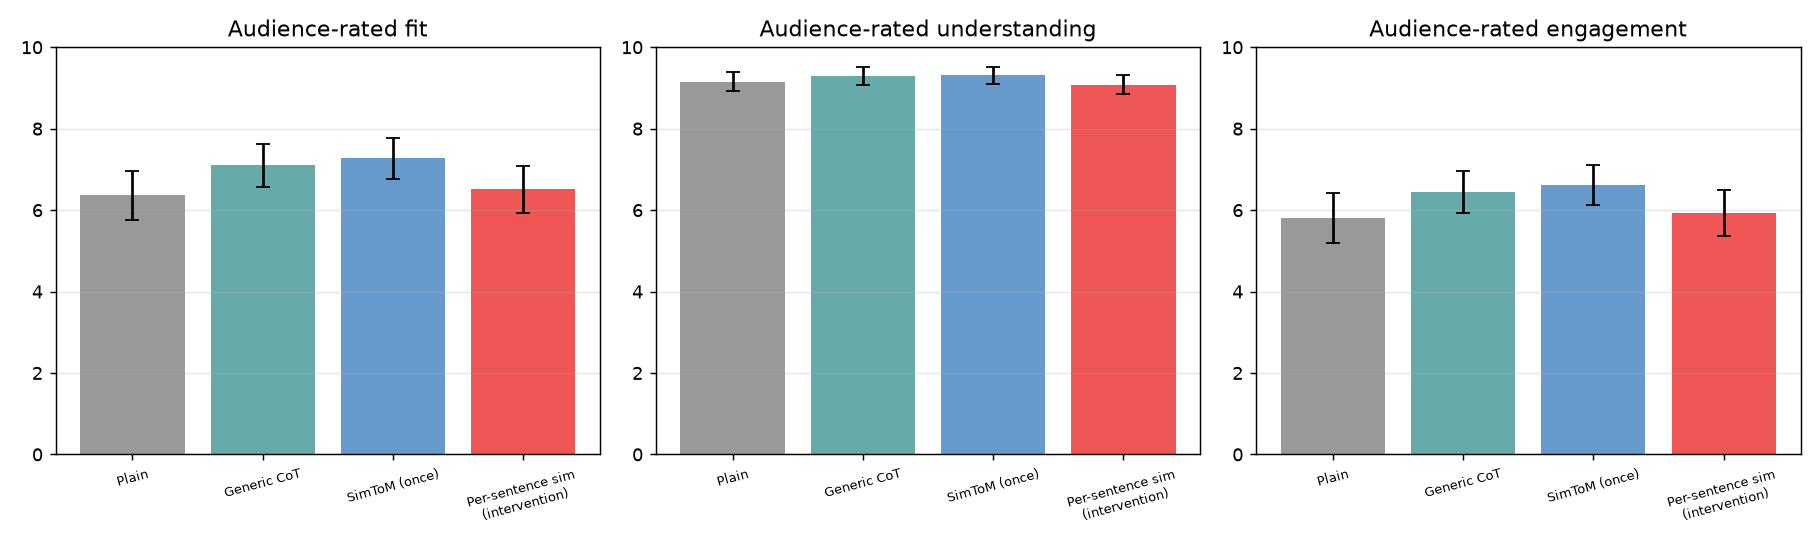
\includegraphics[width=0.6\linewidth]{figures/fig1_absolute_ratings.png}
\caption{Absolute audience ratings with $95\%$ confidence intervals. The intervention
(\persentence) sits near \plain and below both \cot and \simtom on audience fit, engagement, and
understanding; the one-shot audience model \simtom is highest on all three.}
\label{fig:absolute}
\end{figure}

\subsection{Pairwise quality and fit (H2, H4)}
\label{sec:res-pairwise}

\Tabref{tab:pairwise} reports blind, order-balanced pairwise win-rates for the intervention against
each baseline. On \textbf{overall quality} the intervention loses to all three baselines---most
heavily to \simtom, winning only $8.3\%$ of comparisons---and on \textbf{audience fit} it loses to
\cot and \simtom while merely tying \plain. All effects survive Holm correction. Because
\persentence loses to the token-matched \cot control despite both adding reasoning tokens, the
failure is not explained by ``more thinking''---\textbf{H2 and H4 are both refuted}
(\figref{fig:pairwise}).

\begin{table}[t]
\centering
\caption{Pairwise win-rate of \persentence \emph{vs.} each baseline ($n=60$; both orders averaged;
$0.5$ = tie; lower means the intervention loses more often). The intervention loses on overall
quality to \emph{all three} baselines and on audience fit to the two stronger baselines. All
significant win-rates in \textbf{bold}.}
\label{tab:pairwise}
\resizebox{\textwidth}{!}{%
\begin{tabular}{@{}lcc@{}}
\toprule
\textbf{Comparison} & \textbf{Overall quality} (\claude) & \textbf{Audience-fit} (\gemini) \\
\midrule
\persentence vs.\ \plain  & \textbf{0.250} {\scriptsize ($p<0.001$)} & 0.475 {\scriptsize ($p=0.67$, tie)} \\
\persentence vs.\ \cot    & \textbf{0.150} {\scriptsize ($p<0.001$)} & \textbf{0.250} {\scriptsize ($p<0.001$)} \\
\persentence vs.\ \simtom & \textbf{0.083} {\scriptsize ($p<0.001$)} & \textbf{0.200} {\scriptsize ($p<0.001$)} \\
\bottomrule
\end{tabular}%
}
\end{table}

\begin{figure}[t]
\centering
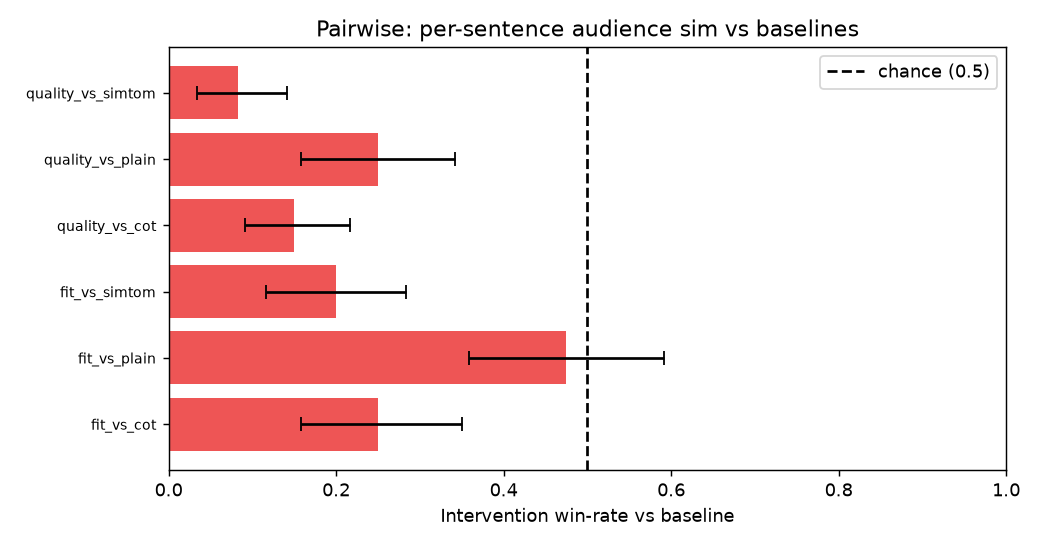
\includegraphics[width=0.6\linewidth]{figures/fig2_pairwise.png}
\caption{Pairwise win-rates for \persentence against each baseline on overall quality and audience
fit. The dashed line marks $0.5$ (tie). Every bar falls below the line: the intervention loses on
quality to all baselines and on fit to \cot and \simtom.}
\label{fig:pairwise}
\end{figure}

\subsection{Does the method actually use the audience? (H3)}
\label{sec:res-adapt}

If per-sentence simulation genuinely tailored writing to the reader, it should show the
\emph{largest} adaptation gap. Instead it shows the \emph{smallest}, tied with \plain
(\Tabref{tab:adapt}). Its gap of $6.04$ is significantly smaller than \simtom's $7.00$
($\Delta=-0.96$, Cohen's $d=-1.27$, $p=0.004$ Holm-corrected) and smaller than \cot's $6.67$
($\Delta=-0.62$, $d=-0.75$). The one-shot audience model, which commits to a single coherent
stance about the reader, adapts \emph{most}. \textbf{H3 is refuted}: the intervention does not use
the audience more---it uses it less (\figref{fig:adapt}).

\begin{table}[t]
\centering
\caption{Adaptation gap (matched-reader minus crossed-reader fit; $n=12$ concepts; higher means
the method tailors more to its intended reader). \persentence has the \emph{smallest} gap,
significantly below \simtom, which has the largest. Best in \textbf{bold}.}
\label{tab:adapt}
\begin{tabular}{@{}lcccc@{}}
\toprule
& \plain & \cot & \simtom & \persentence \textit{(ours)} \\
\midrule
Adaptation gap & 6.08 & 6.67 & \textbf{7.00} & 6.04 \\
\bottomrule
\end{tabular}
\end{table}

\begin{figure}[t]
\centering
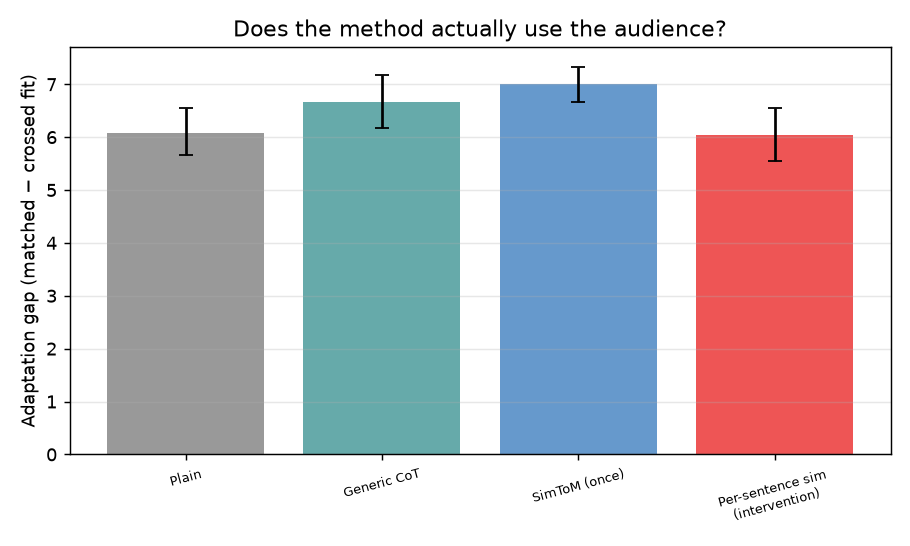
\includegraphics[width=0.6\linewidth]{figures/fig3_adaptation_gap.png}
\caption{Adaptation gap by condition. A larger gap means the method writes differently for
different readers. \persentence adapts \emph{least} (tied with \plain); \simtom adapts most,
contradicting the hypothesis that finer-grained reader simulation yields stronger adaptation.}
\label{fig:adapt}
\end{figure}

\subsection{Homogenization and cost (H5)}
\label{sec:res-cost}

\Tabref{tab:cost} reports diversity and cost. \persentence is the \emph{most} homogenized
condition (highest self-BLEU, lowest distinct-2, tied with \plain) and simultaneously the longest
($170$ words vs.\ $\sim$147) and most token-expensive (2480 thinking characters). \simtom is the
\emph{least} homogenized. So the intervention does not buy diversity with its extra tokens---it
costs the most and produces the most generic prose. \textbf{H5 is refuted}
(\figref{fig:cost}).

\begin{table}[t]
\centering
\caption{Homogenization and cost by condition ($\uparrow$/$\downarrow$ = higher/lower is better).
\persentence is the most homogenized (tied with \plain) \emph{and} the longest and most
token-expensive; \simtom is the least homogenized. Best in \textbf{bold}.}
\label{tab:cost}
\begin{tabular}{@{}lcccc@{}}
\toprule
\textbf{Condition} & distinct-2 $\uparrow$ & self-BLEU $\downarrow$ & words & thinking chars \\
\midrule
\plain        & 0.823 & 0.406 & 148 & 0 \\
\cot          & 0.842 & 0.383 & 144 & 2086 \\
\simtom       & \textbf{0.857} & \textbf{0.363} & 147 & 1762 \\
\persentence \textit{(ours)} & 0.823 & 0.402 & 170 & 2480 \\
\bottomrule
\end{tabular}
\end{table}

\begin{figure}[t]
\centering
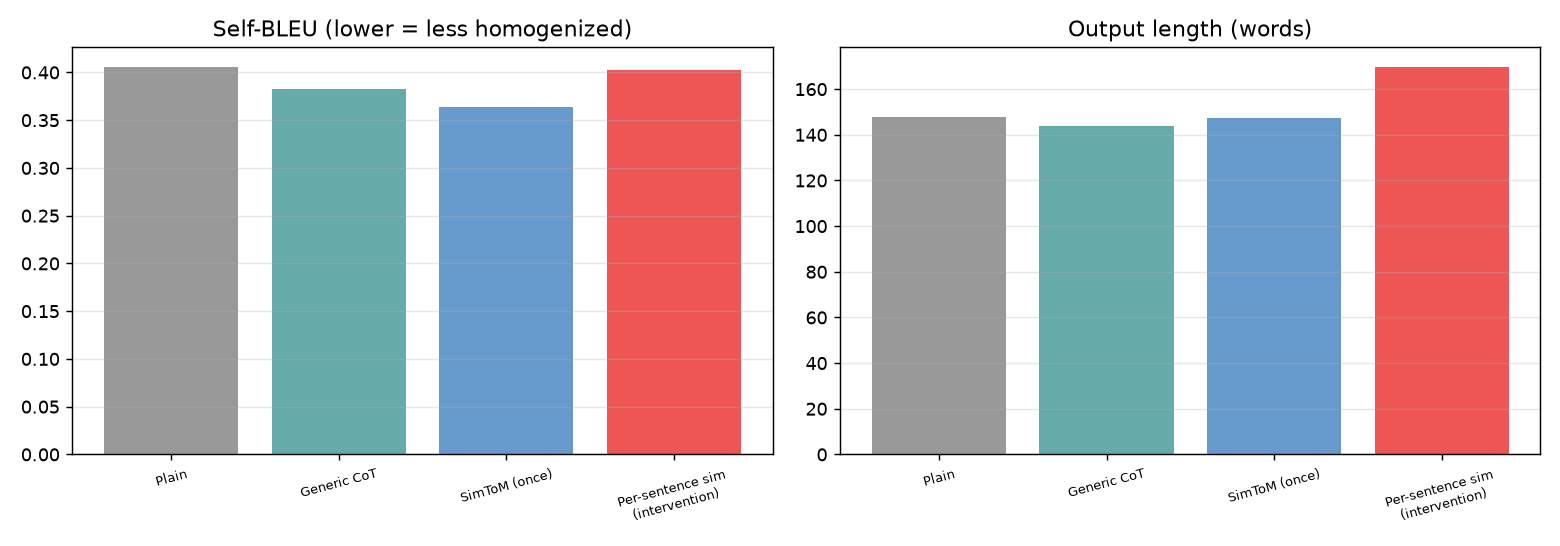
\includegraphics[width=0.6\linewidth]{figures/fig4_diversity_cost.png}
\caption{Diversity and cost. \persentence combines the worst diversity (tied with \plain) with the
highest word count and thinking-token cost, while \simtom achieves the best diversity at lower
cost.}
\label{fig:cost}
\end{figure}

\subsection{Cross-family replication (\llama)}
\label{sec:res-replication}

The same ordering holds with a completely different generator. On the 48 explanatory tasks,
\persentence is worst on fit ($5.52$ vs.\ \simtom/\cot $5.90$) and engagement ($5.02$ vs.\
\simtom $5.46$), and loses pairwise to \emph{every} baseline on both quality (win-rates
$0.115$--$0.260$) and fit (win-rates $0.167$--$0.333$), all significant. The strongest loss is
again to \simtom on quality (win-rate $0.115$, $p<10^{-8}$). The negative result is therefore not
specific to one model family.
